\documentclass[conference]{IEEEtran}
\IEEEoverridecommandlockouts

\usepackage{cite}
\usepackage{amsmath,amssymb,amsfonts}
\usepackage{mathtools}
\usepackage{graphicx}
\usepackage{booktabs}
\usepackage{array}
\usepackage{textcomp}
\usepackage{url}
\usepackage{stfloats}

\graphicspath{{figures/}}

\begin{document}

\title{SpectraForge: A Physics-Grounded, Controllable Benchmark for Band Selection\\
in Multi-Excitation (4D) Fluorescence Hyperspectral Imaging}

% >> author block mirrors the CODASSCA submission; confirm before submitting <<
\author{\IEEEauthorblockN{Narek Meloyan\textsuperscript{1,2,3}, Narine Sarvazyan\textsuperscript{1,3,4}}
\IEEEauthorblockA{\textsuperscript{1}Zaven P.\ and Sonia Akian College of Science and Engineering, American University of Armenia, Yerevan, Armenia\\
\textsuperscript{2}Engineering Research Center, American University of Armenia, Yerevan, Armenia\\
\textsuperscript{3}L.A.\ Orbeli Institute of Physiology NAS RA, Yerevan, Armenia\\
\textsuperscript{4}George Washington University, Washington, DC, USA\\
\texttt{narek\_meloyan@edu.aua.am}, \texttt{phynas@gwu.edu}}}

\maketitle

\begin{abstract}
Multi-excitation fluorescence hyperspectral imaging records, for every pixel, a
four-dimensional excitation-emission cube. Choosing which spectral bands to keep is
central to cheaper acquisition and compact classification, but progress is held back
by a shortage of labeled real data with known ground truth. We present
\textbf{SpectraForge}, an open, physics-grounded generator that renders 4D
excitation-emission cubes from a parametric fluorophore model obeying the standard
laws of fluorescence photophysics (Kasha, Vavilov, Franck-Condon, Stokes shift),
with optional inner-filter attenuation, reabsorption, Foerster resonance energy
transfer (FRET), scatter, photon and read noise, and fixed-pattern clutter. Every
cube carries perfect ground truth, and scenes are built so that band variance is
decoupled from class informativeness (measured correlation $-0.10$), which makes the
benchmark an honest test rather than a trivial one. Alongside the generator we define
an evaluation protocol whose two decisive controls, a random-selection baseline and
the full spectrum, separate genuine gains from self-deception. Using SpectraForge we
characterize autoencoder-plus-latent-perturbation band selection: after correcting a
chance-level published model it reaches 85 to 97 percent of a labels-using oracle,
matches the strongest classical blind selector (PCA loadings) on realistic data, and
\emph{significantly} exceeds it in the nonlinear reabsorption regime (macro-F1
$0.449$ vs $0.431$, $95\%$ CI $[+0.001,+0.029]$). The benchmark also delimits where
unsupervised selection stops helping, and shows that a convolutional model is
structurally necessary when discrimination is spatial. SpectraForge and the full
study are released for reproducible benchmarking in 4D fluorescence imaging.
\end{abstract}

\begin{IEEEkeywords}
hyperspectral imaging, fluorescence, band selection, synthetic benchmark,
autoencoders, excitation-emission, photophysics.
\end{IEEEkeywords}

\section{Introduction}
A multi-excitation hyperspectral cube illuminates a sample at several excitation
wavelengths and, for each, records an emission spectrum across many bands. Every
pixel therefore carries an excitation-emission matrix (EEM), and a scene is a
four-dimensional array over (excitation, emission, height, width). This 4D
fluorescence modality is widely used in biomedical and material imaging because
different fluorophores, tissue states, or species separate in the joint
excitation-emission domain. The per-pixel feature vector (excitations $\times$
emission bands) is high dimensional and largely redundant: only a small subset of
bands carries the information that distinguishes classes. \emph{Band selection}
returns that subset, so a cheaper instrument can acquire only the informative bands
or a downstream classifier can run on a compact feature set.

Developing and comparing band-selection methods for this modality is hampered by a
data problem. Labeled real 4D fluorescence cubes are scarce, and even when available
they have no ground truth: there is no oracle list of which bands truly carry class
information, so a selector cannot be scored against what it should have found.
Synthetic data can supply that ground truth, but only if it is physically faithful
and, critically, only if it does not make the task trivial. In naive synthetic data
the discriminative dyes are also the brightest, so a variance ranker wins and every
method looks good, which tells us nothing.

This paper contributes, first, \textbf{SpectraForge}: an open, physics-grounded,
controllable generator for 4D fluorescence cubes with perfect ground truth, in which
band variance is deliberately decoupled from informativeness. Second, an evaluation
protocol whose random and full-spectrum controls make results honest. Third, a case
study that uses SpectraForge to characterize autoencoder band selection, establishing
both where a learned selector genuinely helps and where simple methods already
suffice. The tool, not any single method, is the durable contribution: it lets the
field benchmark 4D fluorescence band selection on demand and at controllable
difficulty.

\section{The SpectraForge Forward Model}
\subsection{Photophysics}
The generator is grounded in the physics of fluorescence so that ``informative''
means what it means physically. A fluorophore absorbs a photon, relaxes
non-radiatively to the lowest vibrational level of the first excited singlet, and
emits. Four consequences shape the EEM. By \emph{Kasha's rule} emission occurs from
that lowest level regardless of the excitation, so the emission shape is independent
of excitation wavelength and the EEM is approximately trilinear (an excitation
profile times an emission profile times a concentration map), the basis of PARAFAC.
By \emph{Vavilov's rule} the quantum yield is, to first order, independent of
excitation; only the amount absorbed changes. The \emph{Franck-Condon} principle sets
the broadened, roughly mirror-image band envelopes and an optional vibronic shoulder
about $1300\,\mathrm{cm}^{-1}$ to the red. The \emph{Stokes shift} red-shifts emission
relative to absorption.

\subsection{Trilinear render and the additive invariant}
Each fluorophore $k$ is a parametric model with a peak-normalized Gaussian excitation
profile $a_k(\lambda_\mathrm{ex})$ and an area-normalized emission profile
$e_k(\lambda_\mathrm{em})$, extinction $\varepsilon_k$, quantum yield $\Phi_k$, and a
per-pixel concentration map $c_k(x,y)$. The rendered cube is a dilute linear
superposition,
\begin{equation}
F(x,y,\lambda_\mathrm{ex},\lambda_\mathrm{em}) = g \sum_k
c_k(x,y)\,\varepsilon_k\,\Phi_k\,a_k(\lambda_\mathrm{ex})\,e_k(\lambda_\mathrm{em}),
\end{equation}
where $g$ folds lamp, exposure, and power. This is Kasha's rule written as algebra.
With all optional physics and artifacts off the model is \emph{exactly linear},
$\mathrm{render}(A{+}B)=\mathrm{render}(A){+}\mathrm{render}(B)$, an invariant the
implementation tests; difficulty is then added in physically faithful, opt-in
increments. A per-pixel class label is the argmax over the discriminative
fluorophores. Fig.~\ref{fig:fluoro} shows the fluorophore model.

\begin{figure}[t]
\centering
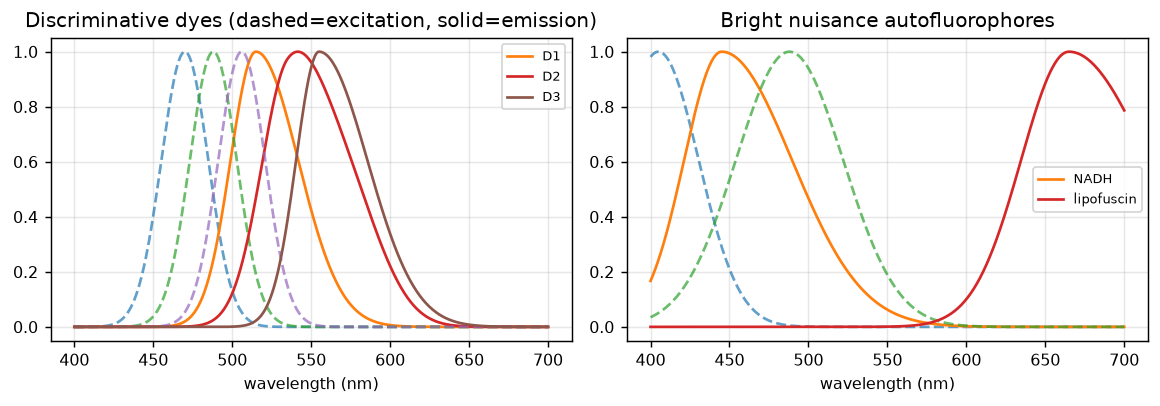
\includegraphics[width=\linewidth]{fig_fluorophores.png}
\caption{Parametric fluorophore spectra. Left: three discriminative dyes (dashed,
excitation; solid, emission) of modest brightness with overlapping emission and
distinct excitation. Right: two bright nuisance autofluorophores that dominate band
variance but carry no class information.}
\label{fig:fluoro}
\end{figure}

\subsection{Variance is decoupled from informativeness}
The central design choice is the scene generator. Discriminative dyes are painted with
smooth random concentration fields whose per-pixel argmax defines the class; these are
dim and spectrally overlapping, so their discriminative content lives in low-variance
band \emph{shape}. Independent nuisance dyes are bright and spatially varying but
class-irrelevant. Real photophysics decouples variance from class in several ways at
once: Rayleigh and Raman scatter ridges are high variance but carry no chemical
identity; bright autofluorescence nuisances add class-irrelevant variance; shot noise
inflates the apparent importance of bright redundant bands; and the discriminative
signal sits in dim or subtly shaped bands. On a confounded SpectraForge scene the
measured correlation between per-band variance and per-band discriminability is
$-0.10$, versus strongly positive on naive clean data. The highest-variance bands
therefore carry no class information (Fig.~\ref{fig:scene}), which is exactly the
property that makes the benchmark an honest test.

\begin{figure*}[t]
\centering
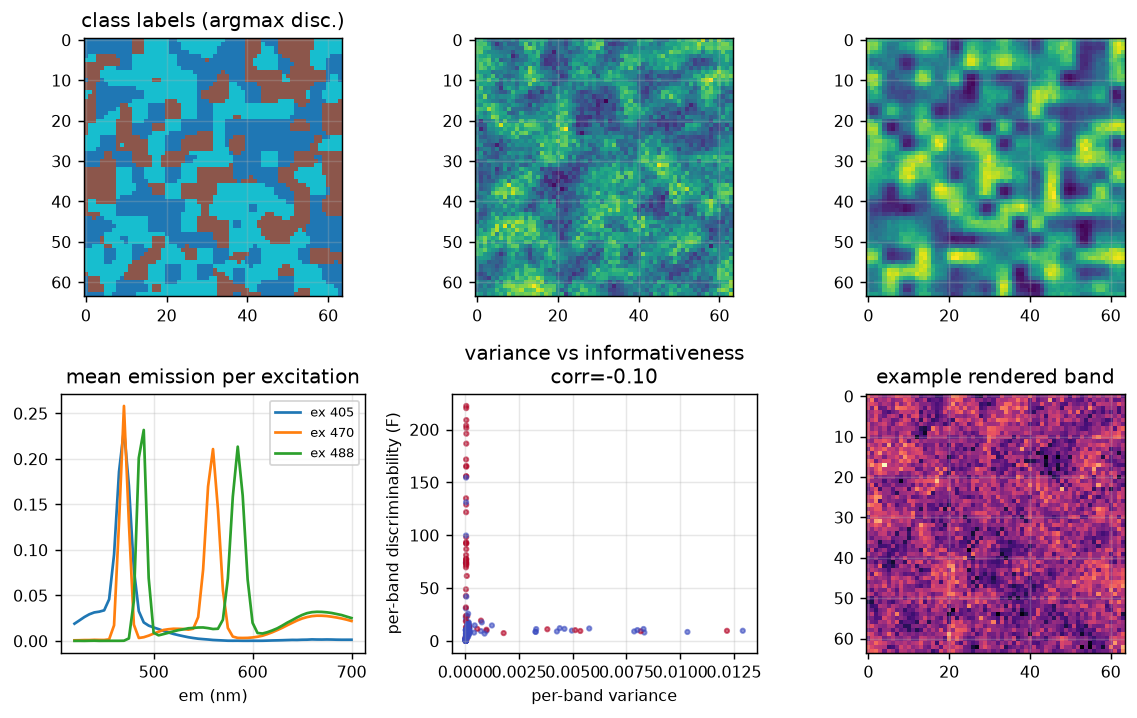
\includegraphics[width=0.92\textwidth]{fig_scene.png}
\caption{The forward model and the variance-versus-informativeness property. Top:
class labels and example rendered bands (a discriminative-dye band, a Rayleigh scatter
band, a nuisance band). Bottom: mean emission per excitation, then the per-band
variance against per-band discriminability (correlation printed near zero), showing
that the loudest bands are not the informative ones.}
\label{fig:scene}
\end{figure*}

\subsection{Artifacts, nonlinear physics, and clutter}
On top of the clean cube the generator adds Rayleigh scatter at
$\lambda_\mathrm{em}=\lambda_\mathrm{ex}$ (with a second-order ghost at
$2\lambda_\mathrm{ex}$) and a water Raman line at a fixed wavenumber offset
($\approx 3400\,\mathrm{cm}^{-1}$), each scaled by a per-pixel turbidity field, then
Poisson shot noise and Gaussian read noise. Three optional effects introduce
concentration nonlinearity: a primary inner filter $\exp(-s A_\mathrm{ex})$;
\emph{reabsorption} $\exp(-s A_\mathrm{em}(\lambda))$, whose overlap with the blue edge
of emission reshapes the band and relocates discriminative information into band shape;
and FRET, where a saturating fraction $E=k c_A/(1+k c_A)$ of donor energy is transferred
to a co-localized acceptor, encoding dye co-localization in a band ratio. Finally,
fixed-pattern clutter injects many class-irrelevant low-rank spatial fields on random
band subsets, the analogue of illumination and detector artifacts and the dominant
real-instrument confound. By dialing these knobs the generator spans \emph{clean}
(variance $\approx$ informativeness), \emph{realistic}, \emph{clutter}, \emph{nonlinear}
(reabsorption or FRET), and \emph{spatial-texture} regimes from a single call.

\subsection{Ground truth, reproducibility, and real fluorophores}
Every render returns a ground-truth sidecar with concentration maps, clean cubes, and
per-fluorophore emission peaks, which enables a tight \emph{peak-recovery} metric
(did a selected band land within a tolerance of a true emission peak; a random selector
scores about $0.33$) in addition to broad information-retention metrics. The generator
exposes a one-call \texttt{build\_dataset} API with explicit knobs for size, emission
sampling, nuisance brightness, scatter, noise, clutter, and nonlinear physics; a script
re-runs every simulation and records exact parameters, so figures and numbers are
reproducible. Parametric dyes can be replaced by real measured spectra imported from
FPbase, and an interactive workbench lets a user paint concentration maps, render, and
validate a selection against ground truth. This makes SpectraForge usable both as a
controlled benchmark and as a design tool for real 4D fluorescence experiments.

\section{Evaluation Protocol}
Selection quality is the accuracy of a downstream classifier trained on the selected
bands, using labels only at evaluation time. We score each subset with a classifier
panel (k-nearest neighbors, random forest, MLP, logistic regression), cross-validated,
reporting macro-F1 and, on nonlinear regimes, a \emph{nonlinear-only gap} (the accuracy
an expressive model recovers beyond a linear one), because a linear metric cannot credit
a nonlinear-shape selection. Two controls are decisive. A \textbf{random} baseline: a
method that cannot beat the $95$th percentile of random band subsets adds nothing. And
the \textbf{full spectrum}: the accuracy ceiling a selector tries to approach. Where
discrimination is spatial we use spatial-block cross-validation to remove
spatial-autocorrelation leakage. These controls, absent from much prior work, are the
difference between an honest result and a self-deception.

\section{Case Study: Autoencoder Band Selection}
The method under study trains an autoencoder to reconstruct the standardized cube,
perturbs each latent dimension, accumulates the per-band reconstruction sensitivity into
a per-band influence, and selects the top-$k$ bands. It is attractive because it is fully
unsupervised yet could in principle capture nonlinear structure that linear methods
(PCA loadings, variance) cannot.

\subsection{From chance to competitive}
Run on modern tooling and scored honestly, the published convolutional model selected at
\emph{chance} (macro-F1 $\approx 0.33$). SpectraForge's ground truth traced this to four
real trainer defects and one architectural flaw. The defects were a library-version crash,
an unbound-variable failure on non-improving loss, a $0\times\mathrm{NaN}$ sparsity term
that silently trained every non-sigmoid run on a NaN loss, and a learning-rate collapse.
The flaw was an emission-axis average-pool that averages away exactly the multi-fluorophore
structure. A misleading per-band $R^2$ metric, dominated by off-peak noise bands, was
replaced by a signal-band correlation whose achievable ceiling is $0.49$, not $1.0$.
Removing the band collapse, and nothing else about the idea, raised reconstruction about
a hundredfold and took selection from chance $0.331$ to $0.414$, about $85\%$ of the
labels-using oracle ($0.486$). Tuning then reached $0.473\pm0.018$ on clean data, matching
the strongest classical blind selector (PCA loadings, $\approx 0.48$) at about $97\%$ of
the oracle. On the confounded regime the debugged selector reaches $0.43$ against a
variance ranker at $0.34$ and a random control at $0.37$, recovering roughly twice as many
true discriminative bands. The benchmark thus both exposed a failure invisible to raw loss
and measured a real recovery.

\subsection{A significance-tested characterization}
A battery of five metric families over eight selectors, multiple regimes, and six seeds,
with bootstrap confidence intervals, places the method precisely (Table~\ref{tab:battery},
Fig.~\ref{fig:results}). The autoencoder \emph{ties} PCA loadings on realistic and FRET
data and \emph{significantly exceeds} it on nonlinear reabsorption (macro-F1 $0.449$ vs
$0.431$, $95\%$ CI $[+0.001,+0.029]$, Cohen $d\approx +0.94$), where its subset carries
nonlinear-only information ($+0.030$) that the linear selector's does not ($-0.021$). PCA
loadings remains the strongest blind selector on clean and linear data, where informative
bands are also the highest-variance ones. The explanation is a general one:
\emph{informative implies has variance implies PCA-selectable}, so a nonlinear
\emph{classification} task does not imply a nonlinear \emph{selection} task; the
autoencoder's manifold advantage helps the downstream classifier, not the band choice.

\begin{table}[t]
\caption{Significance battery: autoencoder vs PCA-loadings (best-of-panel macro-F1,
six seeds). Positive margin favors the autoencoder.}
\label{tab:battery}
\centering
\footnotesize
\setlength{\tabcolsep}{4.5pt}
\renewcommand{\arraystretch}{1.15}
\begin{tabular}{@{}lccc@{}}
\toprule
Regime & AE & PCA-load & margin (95\% CI) \\
\midrule
clean & 0.590 & \textbf{0.635} & $-0.046$ $[-0.079,-0.019]$ \\
realistic & 0.527 & 0.531 & $-0.004$ (tie) \\
reabsorption & \textbf{0.449} & 0.431 & $+0.018$ $[+0.001,+0.029]$ \\
FRET & 0.635 & 0.642 & $-0.007$ (tie) \\
\bottomrule
\end{tabular}
\end{table}

\begin{figure*}[t]
\centering
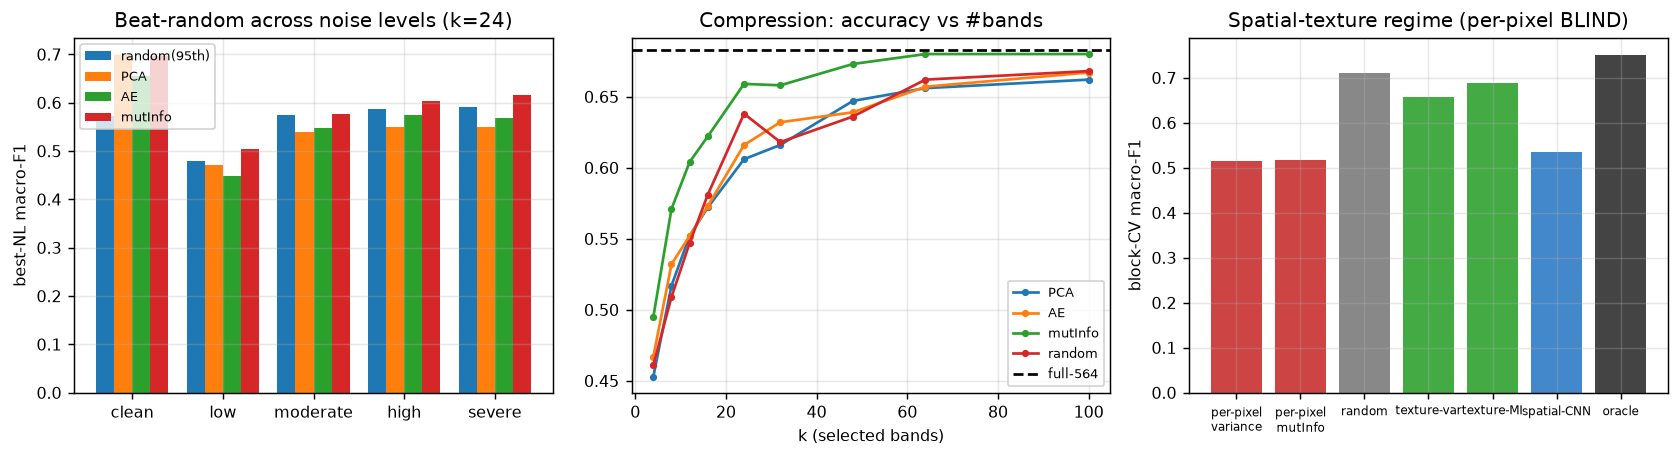
\includegraphics[width=0.98\textwidth]{fig_results.png}
\caption{What SpectraForge reveals. Left: beat-random across five noise levels: blind
PCA and autoencoder selection beat the random $95$th percentile only on clean data, and
under clutter only supervised mutual information does. Middle: compression curve: the
autoencoder tracks PCA at every budget, both reaching about $95\%$ of the full spectrum,
while labels compress about $2.7\times$ better. Right: the spatial-texture regime under
honest block cross-validation: per-pixel selectors are the worst (below random) because
the classes have identical per-pixel spectra, and only a spatial model with the right
bands reaches the oracle.}
\label{fig:results}
\end{figure*}

\subsection{The boundary the benchmark maps}
Because the benchmark includes the two controls, it also delimits where unsupervised
selection stops helping. Under realistic fixed-pattern clutter, blind selection
(autoencoder and PCA alike) does not beat a random subset, because clutter is
high-variance but class-irrelevant, so every variance-driven criterion ranks clutter
bands about randomly with respect to class; there, only label-aware selection beats
random. Across label budgets, selection never beats the full spectrum, so its value is
compression rather than accuracy, and both blind selectors are unstable band by band
(Jaccard $\approx 0.1$ to $0.2$), which argues for selecting spectral regions or
consensus sets. These are not failures of a method but findings of the benchmark:
actionable guidance on when to select bands and when to keep the spectrum.

\subsection{The one structural win: spatial discrimination}
When class is carried by spatial texture, so that every class has the same per-pixel
spectrum, per-pixel band selection is provably blind: under honest block
cross-validation the per-pixel selectors are the worst ($0.52$ to $0.55$, below the
random $0.674$), while a spatial model with the discriminative bands reaches the oracle
($0.78$). This is the one regime where a convolutional model is structurally necessary,
vindicating the original spatial autoencoder idea for spatial classification rather than
for per-pixel spectral band selection.

\section{Discussion and Conclusion}
SpectraForge fills a concrete gap for 4D fluorescence hyperspectral imaging: an open,
physically faithful, controllable source of cubes with perfect ground truth, in which
variance is decoupled from informativeness so that benchmarks are honest rather than
trivial. Paired with a protocol whose random and full-spectrum controls prevent
self-deception, it turns ``does this selector help'' into a measured, reproducible
question. The accompanying case study is a demonstration of that value: it recovers a
chance-level autoencoder to within a few percent of a labels-using oracle, shows a
rigorously significant advantage for learned selection in the nonlinear regime, maps the
clutter boundary where unsupervised selection reduces to a compression tool, and isolates
the spatial regime where a convolutional model is required. The decisive next step is
validation on real Lichens and Collagen cubes with the same controls, where informative
structure need not be variance-prominent. SpectraForge, the evaluation harness, and the
full experiment record are released so that these questions can be studied on shared,
reproducible ground.

\section*{Acknowledgment}
Financial support from the European Union NAS SAR-101087403 and the United States
R44 HL120511 awards is gratefully acknowledged. A large-language-model assistant was
used for code scaffolding, figure generation, and language editing; the design,
analysis, and conclusions are the authors' own and were verified by them.

\begin{thebibliography}{00}
\bibitem{ref_lakowicz} J. R. Lakowicz, \emph{Principles of Fluorescence Spectroscopy},
3rd ed. Springer, 2006.
\bibitem{ref_kasha} M. Kasha, ``Characterization of electronic transitions in complex
molecules,'' \emph{Discuss. Faraday Soc.}, vol.~9, pp.~14--19, 1950.
\bibitem{ref_valeur} B. Valeur and M. N. Berberan-Santos, \emph{Molecular Fluorescence},
2nd ed. Wiley-VCH, 2012.
\bibitem{ref_bro} R. Bro, ``PARAFAC: Tutorial and applications,'' \emph{Chemom. Intell.
Lab. Syst.}, vol.~38, pp.~149--171, 1997.
\bibitem{ref_jablonski} A. Jab\l{}o\'nski, ``Efficiency of anti-Stokes fluorescence in
dyes,'' \emph{Nature}, vol.~131, pp.~839--840, 1933.
\bibitem{ref_hinton} G. E. Hinton and R. R. Salakhutdinov, ``Reducing the dimensionality
of data with neural networks,'' \emph{Science}, vol.~313, pp.~504--507, 2006.
\bibitem{ref_jolliffe} I. T. Jolliffe, \emph{Principal Component Analysis}, 2nd ed.
Springer, 2002.
\bibitem{ref_bsnet} Y. Cai, X. Liu, and Z. Cai, ``BS-Nets: An end-to-end framework for
band selection of hyperspectral image,'' \emph{IEEE Trans. Geosci. Remote Sens.},
vol.~58, no.~3, pp.~1969--1984, 2020.
\end{thebibliography}

\end{document}
